\section{Introduction}

Software relies on state, and many components rely on state machines. For
example, they describe network transport protocols like TCP~\citep{rfc793}, and
implement event-driven systems and regular expression matching.
%
Furthermore, many fundamental resources like network sockets and
files are, implicitly, managed by state machines, in that certain
operations are only valid on resources in certain states, and those operations
can change the states of the underlying resource.  For example, it only makes
sense to send a message on a connected network socket, and closing a socket
changes its state from ``open'' to ``closed''. State machines can also encode
important security properties. For example, in the software which implements
an ATM, it's important that the ATM dispenses cash only when the machine is
in a state where a card has been inserted and the PIN verified.

Despite this, state transitions are generally not checked by compilers.
We routinely use type checkers to ensure that variables and
arguments are used consistently, but statically checking that
operations are performed only on resources in an appropriate state is not well
supported by mainstream type systems.
%
In this paper, we show how to represent state machines precisely in the
dependently typed programming language Idris~\citep{brady2013idris},
and present a library which allows composing larger programs from multiple
state transition systems. The library supports composition in two ways:
firstly, we can use several independently implemented state transition
systems at once; secondly, we can implement one state transition system
in terms of others.

%inspired by the work of Hancock and Setzer on describing
%interactive programming in dependent type theory with command and response
%trees~\citep{hancock-interactive}, and by ongoing work on algebraic effects and
%handlers~\citep{Plotkin2009,Bauer}.  

A motivation for this work is to be able to define communicating
systems, where the type system verifies that each participant follows a 
defined protocol. This is inspired by Session Types~\citep{Honda93,Honda08},
in which the state of a session at any point represents the allowed
interactions on a communication channel. 
%One of the goals, therefore,
%is to represent a form of session types using dependent types. 

However, in order to use session types effectively in practice, we need to be
able to use them in larger systems, interacting with other components. The
\states{} type we present in this paper will allow us to implement a system as
a hierarchy of state machines, and as an example we will implement a
client-server system in which a client requests a random number within a
specific bound from a server, and in which the server processes requests
\emph{asynchronously}. All of the examples are available
online (for review: submitted as supplementary material).

\subsection{Contributions}

We build on previous work on algebraic effects in
Idris~\citep{brady-eff2013,brady-tfp14}. 
In this earlier work, an \emph{effect} is described by an algebraic data
type which gives the operations supported by that effect, and which
is parameterised by a \emph{resource} type.
Operations can change the types of those resources, meaning
that we can implement and verify state transition systems using effects.
However, there are shortcomings: the concrete resource type is defined by the
\emph{effect signature} rather than by its \emph{implementation}; 
it is not possible to create \emph{new} resources in a
controlled way; and, it is not possible to implement \emph{handlers} for
effects in terms of other effects.
%
In this paper, we address these shortcomings, making the following
specific contributions:

\begin{itemize}
\item We present a type, \states{}, which allows a programmer to 
describe a the pre- and post-conditions of a stateful function, creating
and destroying resources as necessary (Section~\ref{sect:statemachines}).
\item We describe the implementation of \states{}, in particular using
Idris' proof automation to construct proofs of correct state management
without programmer intervention (Section~\ref{sect:implementst}).
\item We show how to use \states{} to describe existing stateful APIs,
notably working with network sockets, and to implement high level stateful
systems, such as network application protocols, in terms of these lower level
systems (Section~\ref{sect:examples}).
\end{itemize}

An important goal of \states{} is \emph{usability}, providing notation
to help write \emph{correct} programs without a significant \emph{cost}.
Concretely, this means
that the types need to be readable and need to help direct a programmer to a
working implementation, and error messages need to explain problems clearly. 
We therefore use holes (Section~\ref{sect:getdata})
to help build programs interactively, type level programming
(Section~\ref{sect:sttype}) to provide a readable type level notation, and
error reflection (Section~\ref{sect:errorreflection}) to rewrite error messages
into the language of the problem domain.

Using \states{}, we can encode the assumptions we make about state transitions
in a type, and ensure that these assumptions hold at
run time. Moreover, by allowing state machines to be composed both horizontally
(using multiple state machines at once within a function) and vertically
(implementing a state machine in terms of other, lower level, state machines),
\states{} provides an \emph{architecture} for larger scale dependently typed
programs.

%\subsection{Motivation: Client-Server Communication}

%\label{sect:motivating}

% For each state machine, we use the type system to guarantee that operations
% satisfy their necessary \emph{preconditions}, for example that we can only send
% a reply to a message after receiving a request.  To begin, therefore, 
% we will describe how to represent a state machine in a type, including error
% handling, for a small example: a data store which will only allow data
% to be read after a user has logged in.

\section{Example: A data store, requiring a login}

Our goal is to use the type system not only to describe the inputs
and outputs of functions precisely, but also to explain the effect of
functions on any external resources. 
One way to achieve this is to use an indexed monad~\citep{atkey-param},
where for each operation the monad supports, the type carries a
\remph{precondition} which must hold before the operation is executed,
and a \remph{postcondition} which holds after the operation is executed,
possibly depending on the result of the operation. In a sense, these
are Hoare triples~\citep{hoarelogic}, embedded in the type.
%
In this section, we introduce this idea with a small example: a data store which requires users
to log in before giving access to secret data. 

\subsection{State Transitions in the Store}

The store has two states:
\texttt{LoggedIn}, which means that a user is logged in and able to access
data; and \texttt{LoggedOut}, which means that the user is not logged in.
Reading data is only allowed when the system is in the \texttt{LoggedIn} state.
%
Figure~\ref{fig:login} illustrates the data store, showing the
\remph{states} the system can be in (\texttt{LoggedOut} and \texttt{LoggedIn})
and the operations a user can perform on the system. The operations are:

\begin{itemize}
\item \texttt{login}, which is valid when the system is in the 
\texttt{LoggedOut} state, and either results in the system being in the
\texttt{LoggedIn} state, if login was successful, or the \texttt{LoggedOut}
state otherwise (for example, due to an incorrectly entered password).
\item \texttt{logout}, which is valid when the system is in the
\texttt{LoggedIn} state, and moves the system to the \texttt{LoggedOut} state.
\item \texttt{readSecret}, which returns the data held in the store, and
is only valid when the system is in the \texttt{LoggedIn} state.
\end{itemize}

\begin{figure}[h]
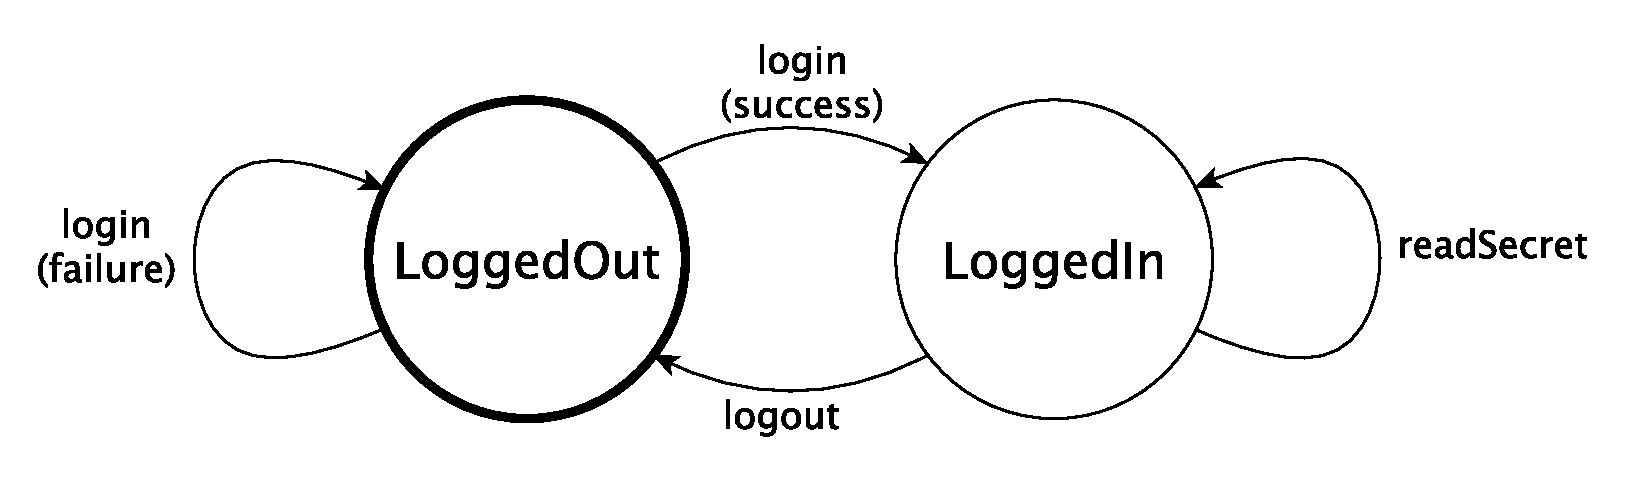
\includegraphics[width=10cm]{diagrams/login.pdf}
\caption{A state machine describing the states and transitions in a system
which allows a program to read some secret data only after successfully logging
in to a data store.}
\label{fig:login}
\end{figure}

By using the type system to capture the state of this system, we can be
sure that a program will only succeed in reading data when it has successfully
logged in to the system. 

\subsection{Representing State Transitions in a Type}

Our goal is that attempting to read data without logging in should result in a
static type error.  Listing~\ref{fig:storemonad} shows how we can achieve this
using an indexed monad.

\small
\begin{code}[float=h, frame=single,caption={Implementing the state store as
an indexed monad},label=fig:storemonad]
data Access = LoggedOut | LoggedIn
data LoginResult = OK | BadPassword

data Store : (ty : Type) -> Access -> (ty -> Access) -> Type where
     Login : Store LoginResult LoggedOut
                   (\res => case res of
                                 OK =>          LoggedIn
                                 BadPassword => LoggedOut)
     Logout :     Store ()     LoggedIn  (const LoggedOut)
     ReadSecret : Store String LoggedIn  (const LoggedIn)

     Pure : (x : ty) -> Store ty (st x) st
     Lift : IO ty -> Store ty st (const st)
     (>>=) : Store a st1 st2 -> ((x : a) -> Store b (st2 x) st3) -> Store b st1 st3
\end{code}
\normalsize

The \texttt{Store} indexed by the type of the result of the operation, the
required input state, and an output state calculated from the result of the
operation. In the simplest cases, such as \texttt{Logout}, the result has no
influence on the result, so we use \texttt{const} (which returns its first
argument and discards its second) to compute the result state:

\small
\begin{code}
Logout : Store () LoggedIn (const LoggedOut)
\end{code}
\normalsize

When we \texttt{Login}, on the other hand, the result state depends on the
result of the operation. If login is successful, it returns \texttt{OK},
and the resulting state of the system is \texttt{LoggedIn}; otherwise, it
is \texttt{LoggedOut}:

\small
\begin{code}
Login : Store LoginResult LoggedOut (\res => case res of
                                                  OK =>          LoggedIn
                                                  BadPassword => LoggedOut)
\end{code}
\normalsize

\subsection{Implementing a program to access the \texttt{Store}}

\label{sect:getdata}

Listing~\ref{fig:storeprog} shows how to combine operations on the store into a
complete function which attempts to login, then reads and prints the data if
successful, or prints an error if not.

\small
\begin{code}[float=h, frame=single,caption={A function which logs in to the
store and reads the secret data if login succeeds},label=fig:storeprog]
getData : Store () LoggedOut (const LoggedOut)
getData = do result <- Login
             case result of
                  OK => do secret <- ReadSecret
                           Lift (putStr ("Secret: " ++ show secret ++ "\n"))
                           Logout
                  BadPassword => Lift (putStr "Failure\n")
\end{code}
\normalsize

Rather than writing \texttt{getData} in one go, we develop it interactively
using \emph{holes}. The following listing contains a hole
\texttt{getData\_rest}, which stands for the rest of the sequence after
attempting to login:

\small
\begin{code}
getData : Store () LoggedOut (const LoggedOut)
getData = do result <- Login
             ?getData_rest
\end{code}
\normalsize

Then, if we check the type of the hole, we can see both the current state of
the system explicitly in the type, and the required state at the end of the
function. Here, we see we need to inspect \texttt{result}:

\small
\begin{code}
getData_rest : Store () (case result of
                              OK => LoggedIn
                              BadPassword => LoggedOut) (const LoggedOut)
\end{code}
\normalsize

%The type here indicates that we can only make progress 
%by inspecting the value of \texttt{result}.
%Functions with holes can be type checked, and even compiled, although
%executing an incomplete program gives a run time error.

We leave \remph{execution} of a \texttt{Store} program abstract here;
this depends on factors such as how to connect to the store, the security
policy, and so on.
Nevertheless, by defining an indexed monad for the operations on a data store,
we can be sure that programs which access the store correctly follow a protocol
of logging in before reading data. However, there are limitations to this
approach. For example:

\begin{itemize}
\item What if we want to write programs which use other external 
resources, as well as the data store?
\item % What if we need access to several different stores? 
Can we connect to an arbitrary number of stores, rather than being limited to
one?
\item \texttt{Store} describes a session with a
\remph{connected} store. How do we handle connecting and disconnecting?
\end{itemize}

In the rest of this paper, we will decribe a library, \states{}, written in
Idris, which allows us to describe APIs such as those provided by
\texttt{Store}.  It will address the above limitations, allowing us to
\remph{compose} multiple stateful systems, implement systems in terms of other,
lower level systems, and create and destroy resources as required.

\endinput

\endinput

\begin{figure}
\begin{center}
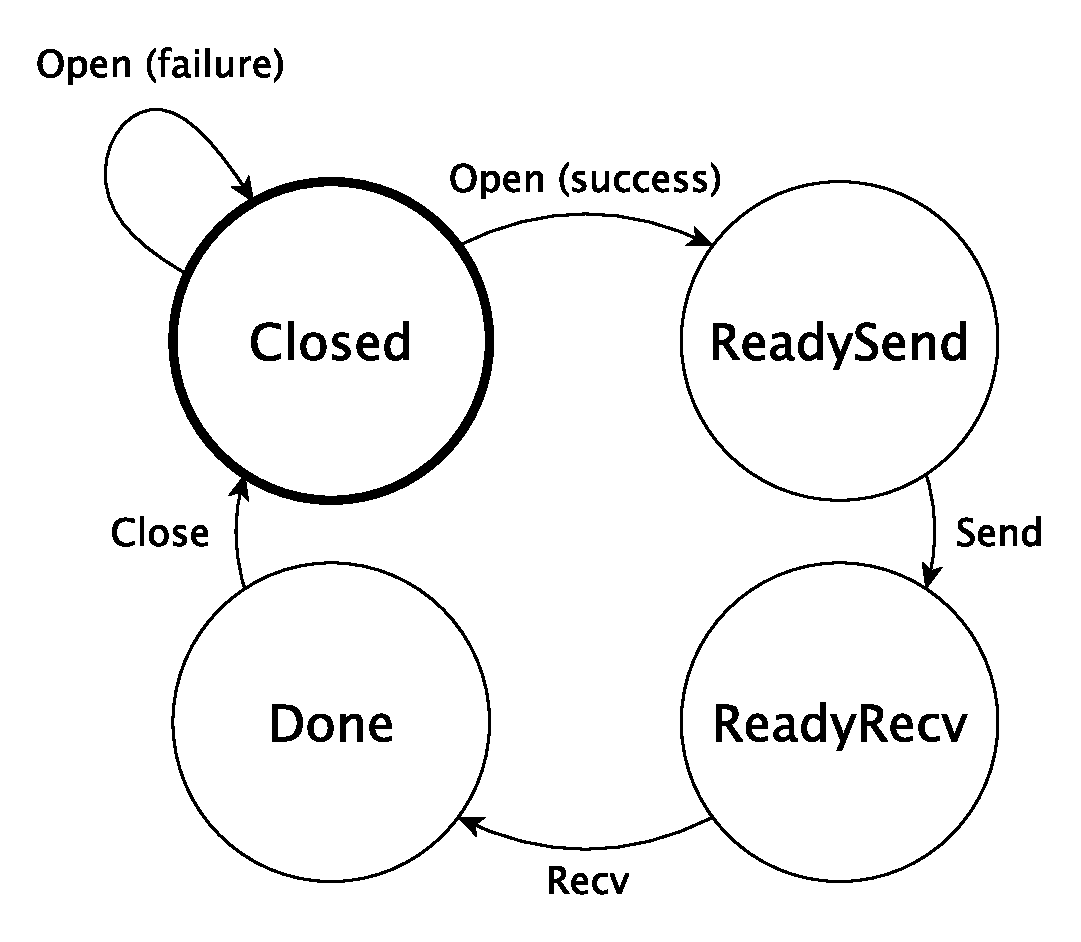
\includegraphics[width=7cm]{diagrams/randclient.pdf}
\end{center}
\caption{A state transition diagram which shows the states and
operations of a client which connects to a server, sends a single message
    and receives a reply. The initial and final state is \texttt{Closed}.}
\label{fig:randclient}
\end{figure}

Figure~\ref{fig:randclient} shows the general form of the states in a
client, where the client connects to a server, sends a message, waits for
a reply, then closes the connection.
Connecting to the server may fail, for example due to a network error, so
in practice we'll need to check whether the \tFN{Open} operation was
successful. Furthermore, although we may have implemented the client
correctly, we can't assume that the server is implemented correctly. If the
server is following a different protocol, \tFN{Recv} may also fail.

\begin{figure}
\begin{center}
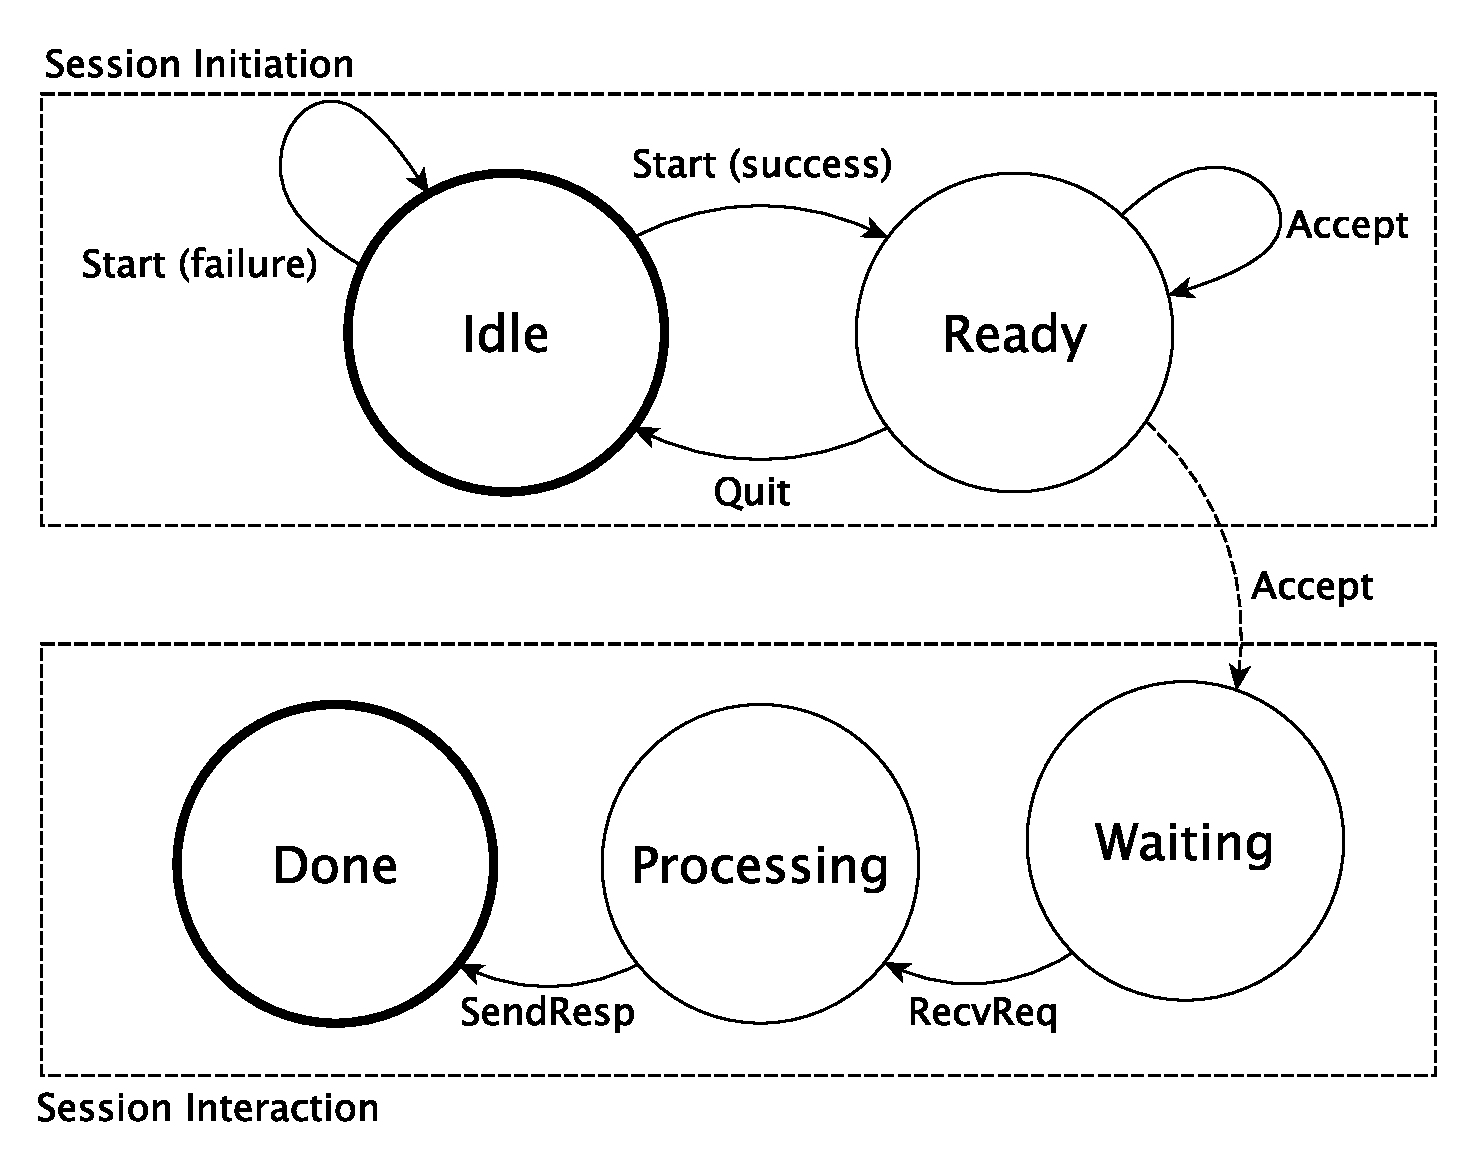
\includegraphics[width=9cm]{diagrams/randserver.pdf}
\end{center}
\caption{A state transition diagram which shows the states and
operations of a server which waits for connections from a client.
    On accepting a connection, it also starts a new machine in the \texttt{Waiting}
    state. The initial state is \texttt{Idle} and the final states are
    \texttt{Idle} and \texttt{Done}.}
\label{fig:randserver}
\end{figure}

A client only has to deal with one connection, to a single server. A server, on
the other hand, may receive requests from several clients. 
Figure~\ref{fig:randserver} shows the general form of the states in a server
which waits for connections from clients, and on receiving a connection
initiates a session in which it waits for an incoming message, then sends
a reply. When it initiates a session, the session itself might run in 
another thread or process. There are two state machines here:

\begin{enumerate}
\item \textbf{Session initiation:} either the server is not running, or it's ready
for an incoming connection. When it receives an incoming connection, it
sets up a new \emph{session interaction} state machine for that connection
and continues waiting for connections
\item \textbf{Session interaction:} the session waits for an incoming message,
processes that message and sends a response, then the session is complete
\end{enumerate}

